\chapter{Low Power, yet Powerful}\label{benchmark}
The ARM-based processors have received great attention for its characteristic of low power consumption and energy efficiency, especially in smart phone and portable device industry, where power consumption is one the most critical specifications. Furthermore, there is trend in server industry to shift to ARM-based architecture in order to cut off the bill of electricity. ARM is also ambitious in this area and about to publicize processors capable of virtualization. When it comes to rural development, power shortage has been forcing researchers and engineers to seek for alternative power sources. Lower power consumption of the equipments implies a bigger potential of surviving severe environment.
Currently, we are exploring the possibilities of two platforms, namely Raspberry Pi and Odroid. The specifications of these two platform can be found in Table X
%TODO specification table
In the following sections, we benchmark a variety of attributes of Odroid and Raspberry Pi. The objective is to clarify the capacity of these two platforms and an optimum form to run the web service. We test every component of a complete Moodle installation to identify the bottleneck of the application. Based on the results, we propose the optimum cluster solution that can be easily scaled out to serve more users.

%\section{Processor and Bandwidth Latency}
\section{Benchmark of Web Components}
To test components of a complete Moodle installation, we design a expirement in Figure X. Each part is respectively substituted with either Odroid or Raspberry Pi, and remaining parts are running on a high-end machine which is much more powerful than these two platforms, in order to put enough siege on the testing target. Furthermore, simulated requests are generated from high-end machine as well.

\subsection{Web Frontend}
Most of the websites today are powered by Apache due to its long history and abundant extensions. Although Apache relies on a processed-based manner to handle new connection, which has limited the scalability and concurrency. Nginx is an event-based reverse proxy that handles request asynchronizily. It addresses C10K problem from the beginning and focus on scalability.
To determine which server runs better on a resource constraint platform, we benchmark Nginx and Apache on both platform to evaluate the throughput, level of concurrency and response delay. We use siege to generate workload and compare the performance of web server with two different type of object: small text file and large JPG file.
We siege the server in following setting:
%TODO topology

\begin{figure}[h]
\centering
\begin{subfigure}{0.45\textwidth}
\centering
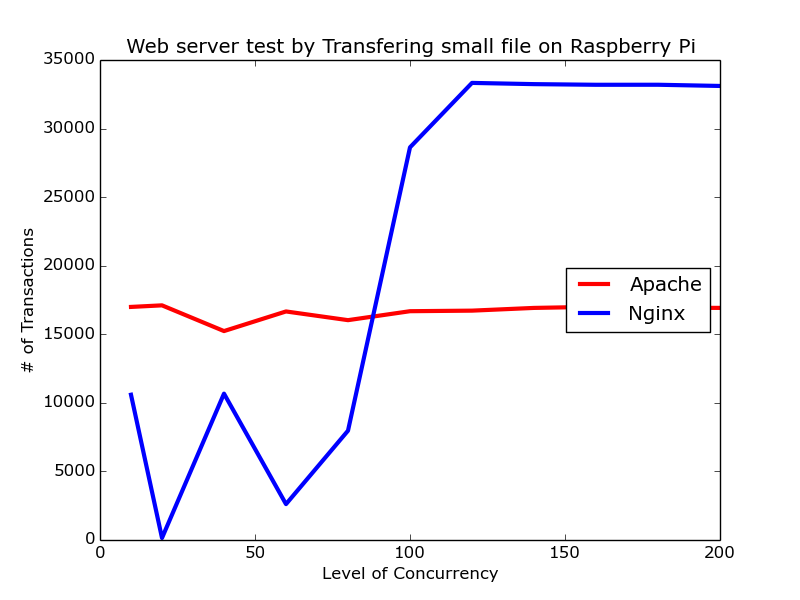
\includegraphics[width=\textwidth]{rpi_small_text.png}
\caption{Raspberry Pi (small text file)}
\end{subfigure}
\begin{subfigure}{0.45\textwidth}
\centering
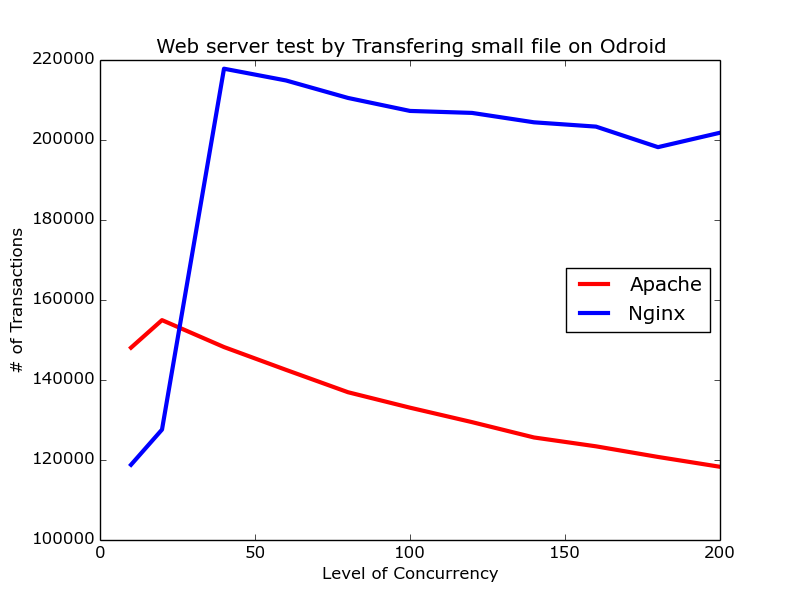
\includegraphics[width=\textwidth]{odroid_small_text.png}
\caption{Odroid (small text file)}
\end{subfigure}

\begin{subfigure}{0.45\textwidth}
\centering
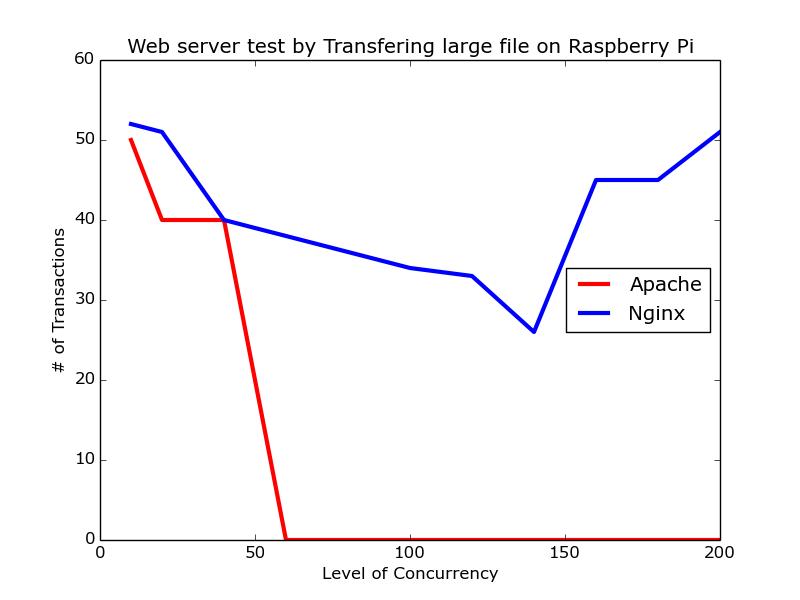
\includegraphics[width=\textwidth]{rpi_big_jpg.png}
\caption{Raspberry Pi (big jpg file)}
\end{subfigure}
\begin{subfigure}{0.45\textwidth}
\centering
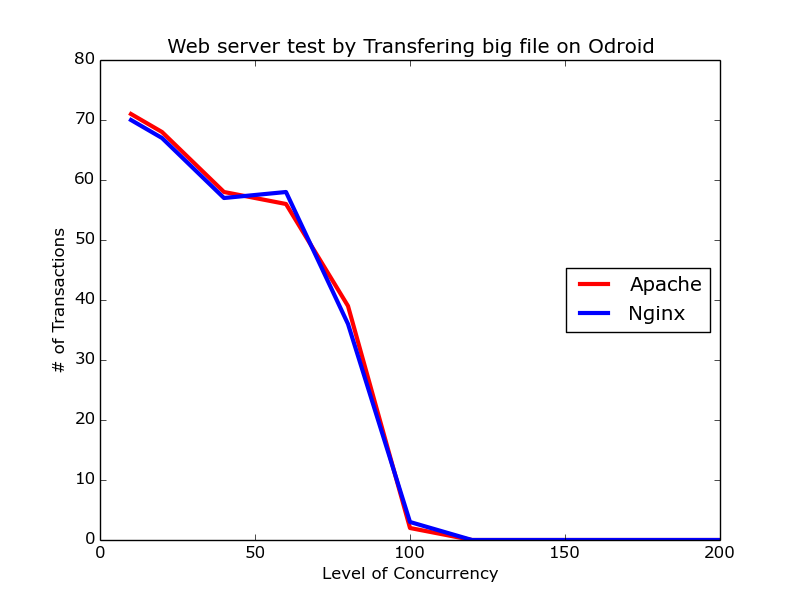
\includegraphics[width=\textwidth]{odroid_big_jpg.png}
\caption{Odroid (big jpg file)}
\end{subfigure}
\caption{A Benchmark of static file request on both platforms}
\label{static}
\end{figure}

As shown if Figure \ref{static}, Nginx and Apache achieve comparable performance under a low level of concurrency, although Nginx outperforms Apache notebly when concurrency level increases. To be noticed, both web servers perform indistinguishably while serving large file. We observe fully occupied CPU in this specific test, which is due to intensive OS kernel processing of socket manipulation and packet tranfer. The impact of web server on the CPU is neglectable in this circumstance. Thus, expirement result in Figure \ref{static}(d) does not denote same performance of web servers.

\subsection{PHP Processing}
As a large PHP application, Moodle requires significant computational resources for PHP processing. Thus, a testbed is formed to benchmark PHP processing capacity of two platforms, see Figure X
%TODO PHP benchmark testbed
The inputs are two different PHP scripts:
\begin{itemize}
\item a php script simply echoes \texttt{Hello, world!}
\item Moodle index page which requires heavy php processing.
\end{itemize}

\begin{figure}[h]
\centering
\begin{subfigure}{0.45\textwidth}
\centering
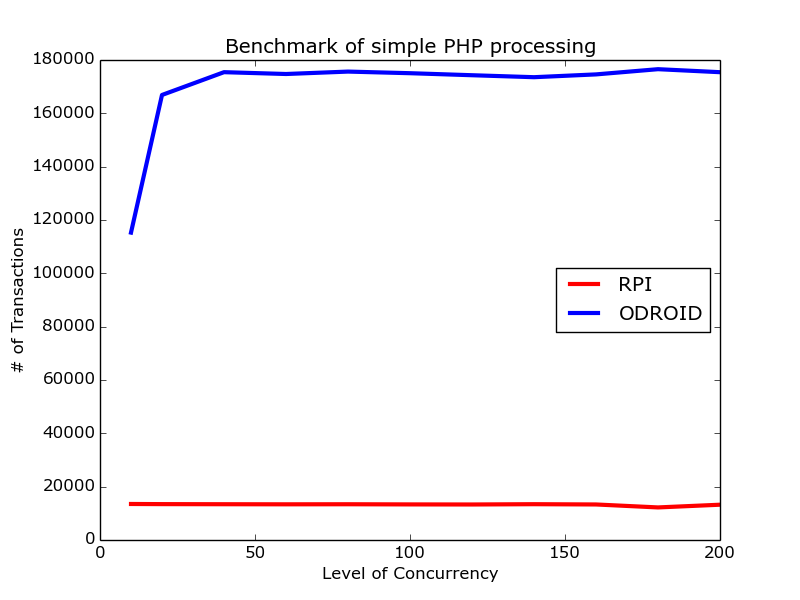
\includegraphics[width=\textwidth]{simple_php.png}
\caption{$\sum trans$}
\end{subfigure}
\begin{subfigure}{0.45\textwidth}
\centering
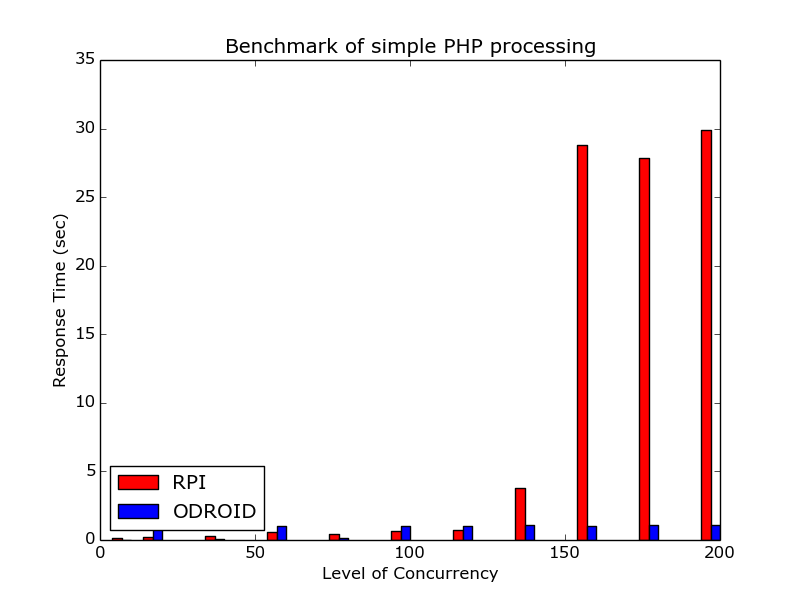
\includegraphics[width=\textwidth]{simple_php_max_res.png}
\caption{Longest Response Time}
\end{subfigure}
\caption{A Benchmark of simple PHP processing on both platforms}
\label{simple_php}
\end{figure}

Figure \ref{simple_php}(a) shows that Odroid can handle much more PHP request than Raspberry Pi. Overall response time is shorter for Odroid. Although, half of the CPU usage is taken by OS kernel during these two test and the difference satisfactorily convincing. The gap between two platforms is more evident when tested with heavier PHP processing, as shown in Figure \ref{moodle_php_result}.\footnote{We observe a 6~7 seconds delay to process index page of Moodle on Raspberry Pi and it can barely tolerate the mildest siege. Thus, the test result of Raspberry Pi is left out in this test.}

\begin{figure}[h]
\centering
\begin{subfigure}{0.45\textwidth}
\centering
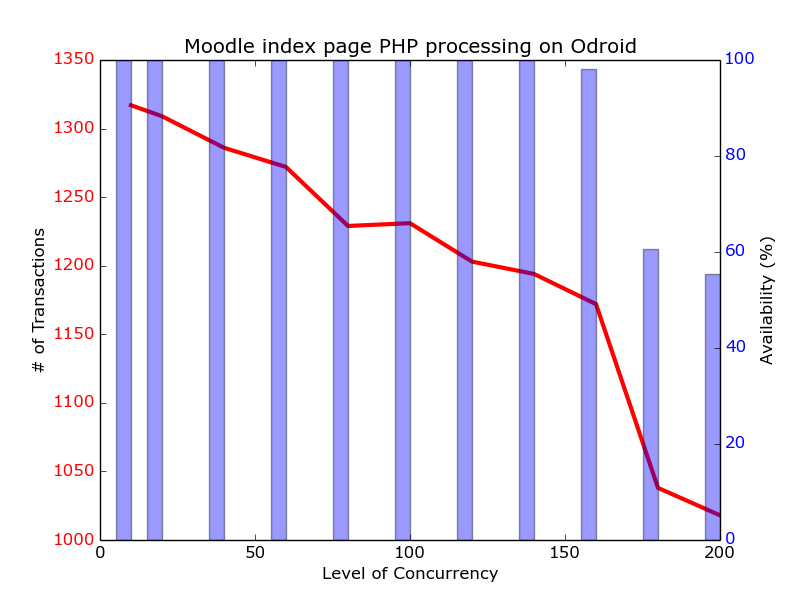
\includegraphics[width=\textwidth]{moodle_index.png}
\caption{$\sum trans$ \& Availability}
\end{subfigure}
\begin{subfigure}{0.45\textwidth}
\centering
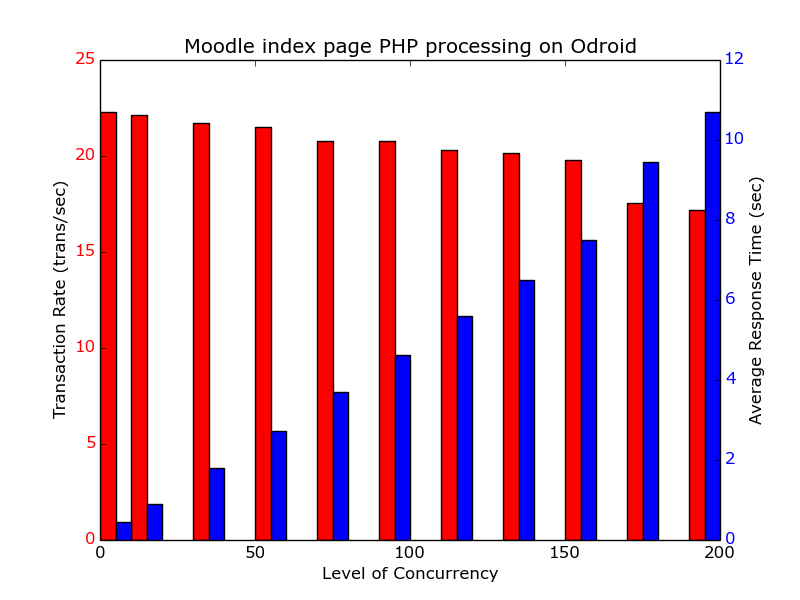
\includegraphics[width=\textwidth]{moodle_index_2.png}
\caption{$Rate_{trans}$ \& $T_{resp}$}
\end{subfigure}
\caption{Moodle index processing on Odroid}
\label{moodle_php_result}
\end{figure}

As shown in Figure\ref{moodle_php_result}(a), transaction rate and availability drops under 180 concurrent requests occur. The latency is beyond tolerable under 50 concurrent requests, according to a study of tolerable waiting time of website\ref{nah2004study}. As the total transaction number in this test is significantly lower than the previous one in Figure \ref{simple_php}, we suspect that PHP processing power is the bottleneck in a moodle installation rather than database query and web frontend. Thus, we test the capacity of a standalone installation of Moodle, in which all components are in one box (Odroid), shown in Figure \ref{standalone}.

\begin{figure}[h]
\centering
\begin{subfigure}{0.45\textwidth}
\centering
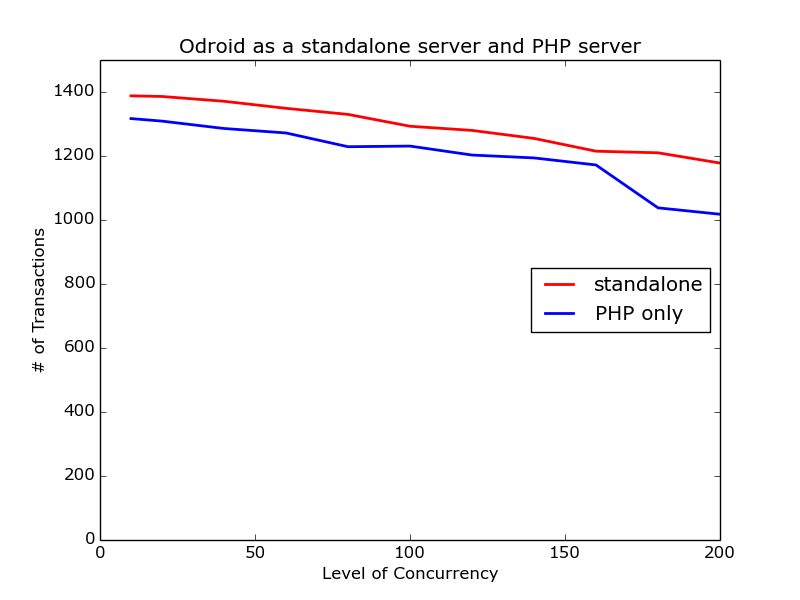
\includegraphics[width=\textwidth]{standalone.png}
\caption{$\sum trans$ \& Availability}
\end{subfigure}
\begin{subfigure}{0.45\textwidth}
\centering
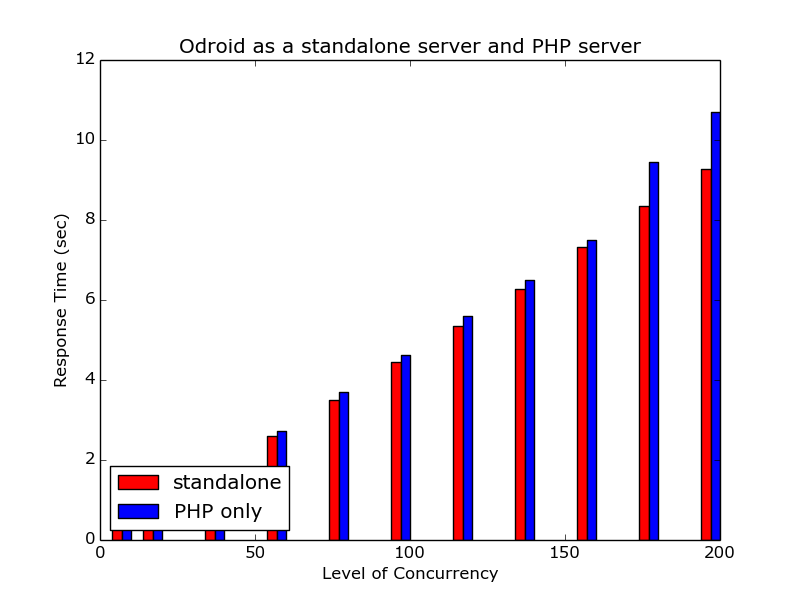
\includegraphics[width=\textwidth]{standalone_res.png}
\caption{$T_{resp}$}
\end{subfigure}
\caption{Odroid as a standalone server and PHP server}
\label{standalone}
\end{figure}

Impact of adding web frontend does not evidently influence transaction rate, which implies that PHP processing capacity is the limiting factor in one Moodle installation.

\subsection{Database}
We apply the same method to test database although fail to exhaust the resource on Odroid before running out CPU and memory on our testbed high-end machine, hence we conclud that database query does not limit a Moodle installation before expanding PHP capacity.

\section{Scale Out to Eliminate Bottleneck}
To benefit most from currently available hardwares, we propose to form a small scale cluster than can be easily scaled out to cope with an increase of users. Furthermore, we investigate multiple different formations to find out the most economical setting. An intuitive solution is to put different services in physically separated hardwares, as a structure shown in Figure \ref{naive_cluster_form}. Nginx server in Rapsberry Pi features both web server and load balancer with upstream PHP servers running in Odroid. To cope with the increase of users, this setting can be easily scaled out by simply adding more hardware for PHP processing.
%TODO naive_cluster figure
\begin{figure}[htbp]
\centering
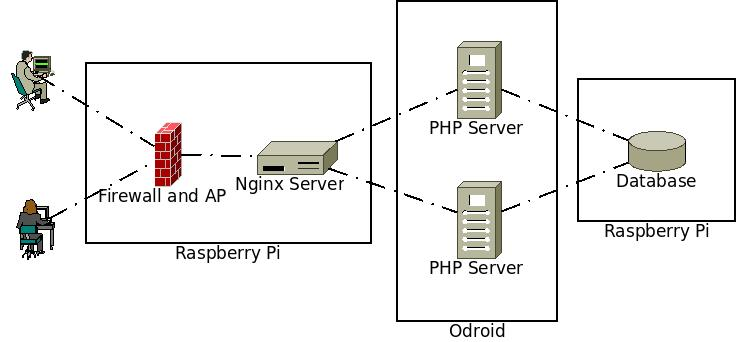
\includegraphics[width=0.9\textwidth]{naive_cluster.jpeg}
\caption{A naive form of cluster}
\label{naive_cluster_form}
\end{figure}
Although, as we compare the Siege test result with a standalone installation where all services run in one Odroid, we encounter a slightly lower performance, which is even worsen after we add one more PHP server, see Figure \ref{naive_cluster}.

\begin{figure}[htbp]
\centering
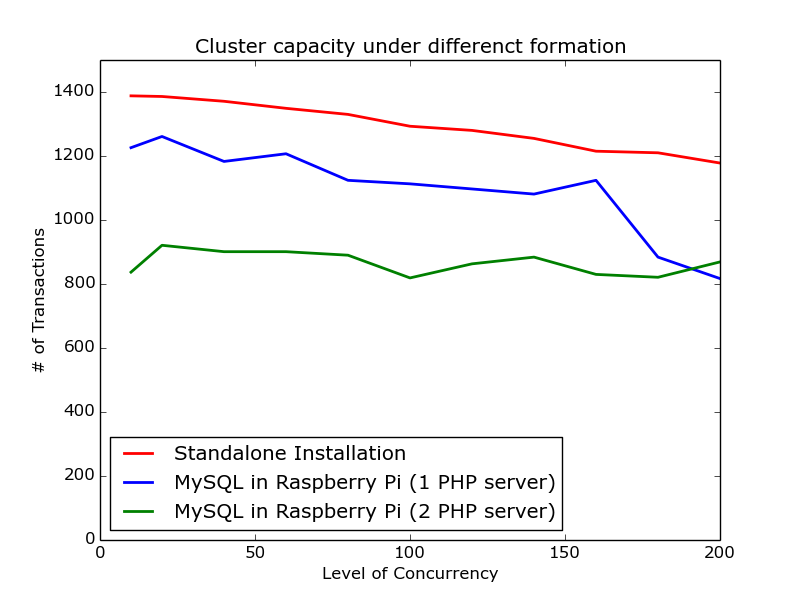
\includegraphics[width=0.5\textwidth]{naive_cluster.png}
\caption{The Performance of running Database in Raspberry Pi}
\label{naive_cluster}
\end{figure}

To further identify the cause, we siege the cluster with 100 simulated concurrent clietns and observe CPU usage of servers (CPU of Nginx server is far from full load hence left out in the result), the result is shown in Figure \ref{cpu_usage}. We deduce that most of CPU resource in database server is consumed by OS kernel to handle concurrent sockets.
\begin{figure}[htbp]
\centering
\begin{subfigure}{0.45\textwidth}
\centering
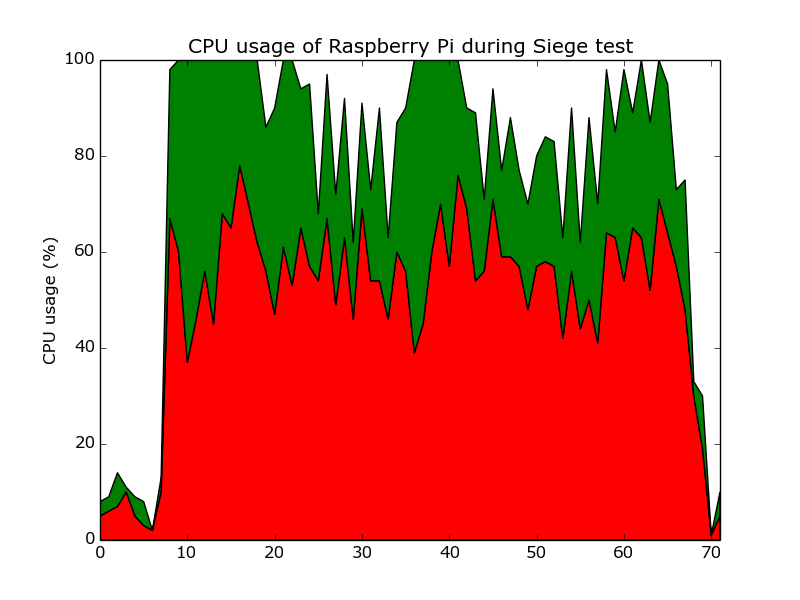
\includegraphics[width=\textwidth]{cpusage_rpi.png}
\caption{database}
\end{subfigure}
\begin{subfigure}{0.45\textwidth}
\centering
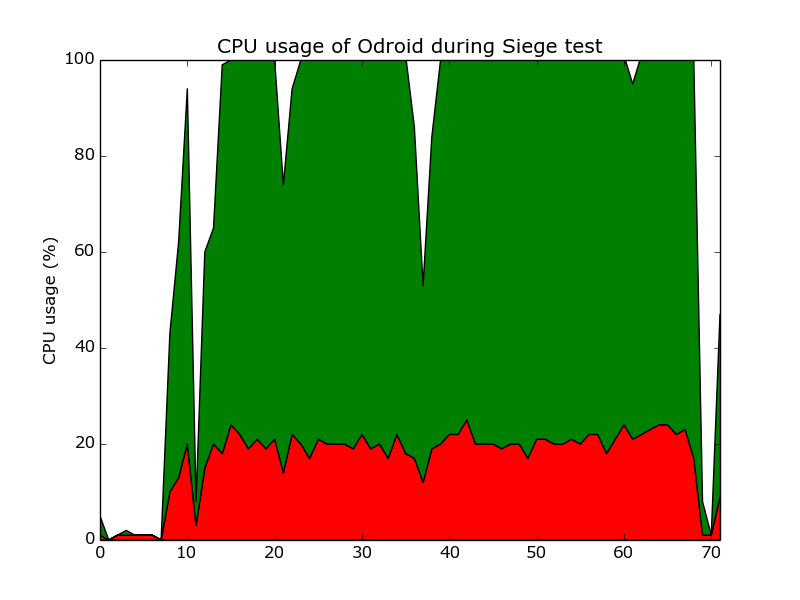
\includegraphics[width=\textwidth]{cpusage_odr.png}
\caption{PHP}
\end{subfigure}
\caption{CPU usage of servers}
\label{cpu_usage}
\end{figure}

Hence, database needs to be more closely coupled with PHP server, which results in the cluster formation in Figure \ref{good_cluster}. And the result meets our assumption that server capacity improves by adding extra PHP server, see Figure \ref{good_cluster_perf}

\begin{figure}[h]
\centering
\begin{subfigure}{0.7\textwidth}
\centering
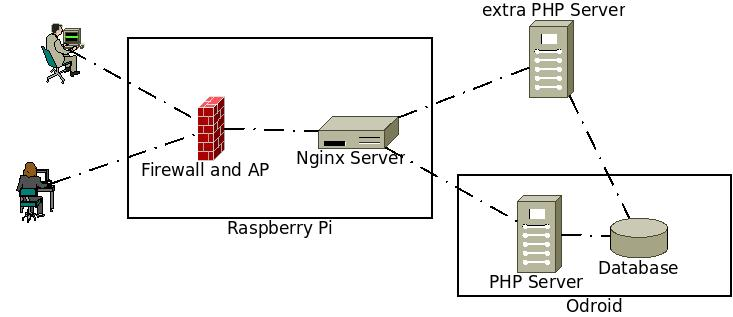
\includegraphics[width=\textwidth]{clever_cluster.jpeg}
\caption{A better form of cluster}
\label{good_cluster}
\end{subfigure}

\begin{subfigure}{0.45\textwidth}
\centering
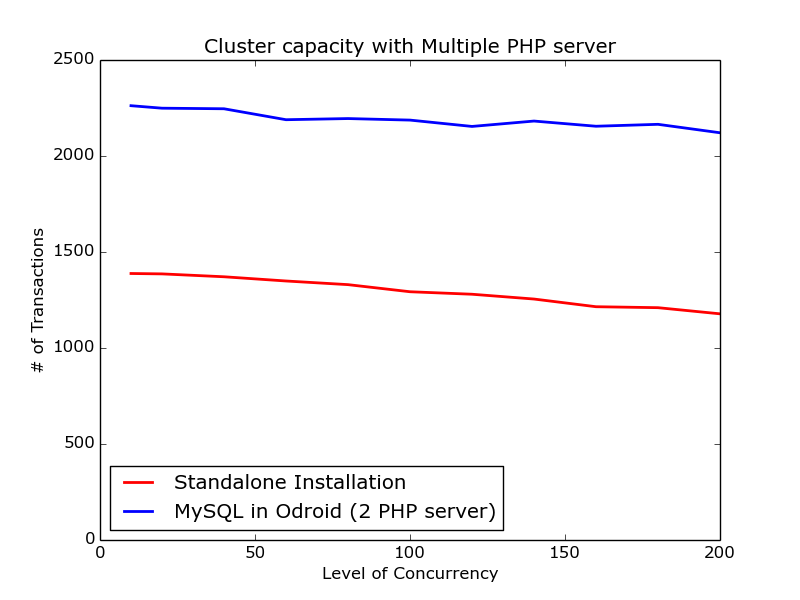
\includegraphics[width=\textwidth]{clever_cluster.png}
\caption{Performance of cluster with multiple PHP servers}
\label{good_cluster_perf}
\end{subfigure}
\end{figure}



